%Lab 5 Write Up


\documentclass{article}\usepackage[]{graphicx}\usepackage[]{xcolor}
% maxwidth is the original width if it is less than linewidth
% otherwise use linewidth (to make sure the graphics do not exceed the margin)
\makeatletter
\def\maxwidth{ %
  \ifdim\Gin@nat@width>\linewidth
    \linewidth
  \else
    \Gin@nat@width
  \fi
}
\makeatother

\definecolor{fgcolor}{rgb}{0.345, 0.345, 0.345}
\newcommand{\hlnum}[1]{\textcolor[rgb]{0.686,0.059,0.569}{#1}}%
\newcommand{\hlsng}[1]{\textcolor[rgb]{0.192,0.494,0.8}{#1}}%
\newcommand{\hlcom}[1]{\textcolor[rgb]{0.678,0.584,0.686}{\textit{#1}}}%
\newcommand{\hlopt}[1]{\textcolor[rgb]{0,0,0}{#1}}%
\newcommand{\hldef}[1]{\textcolor[rgb]{0.345,0.345,0.345}{#1}}%
\newcommand{\hlkwa}[1]{\textcolor[rgb]{0.161,0.373,0.58}{\textbf{#1}}}%
\newcommand{\hlkwb}[1]{\textcolor[rgb]{0.69,0.353,0.396}{#1}}%
\newcommand{\hlkwc}[1]{\textcolor[rgb]{0.333,0.667,0.333}{#1}}%
\newcommand{\hlkwd}[1]{\textcolor[rgb]{0.737,0.353,0.396}{\textbf{#1}}}%
\let\hlipl\hlkwb

\usepackage{framed}
\makeatletter
\newenvironment{kframe}{%
 \def\at@end@of@kframe{}%
 \ifinner\ifhmode%
  \def\at@end@of@kframe{\end{minipage}}%
  \begin{minipage}{\columnwidth}%
 \fi\fi%
 \def\FrameCommand##1{\hskip\@totalleftmargin \hskip-\fboxsep
 \colorbox{shadecolor}{##1}\hskip-\fboxsep
     % There is no \\@totalrightmargin, so:
     \hskip-\linewidth \hskip-\@totalleftmargin \hskip\columnwidth}%
 \MakeFramed {\advance\hsize-\width
   \@totalleftmargin\z@ \linewidth\hsize
   \@setminipage}}%
 {\par\unskip\endMakeFramed%
 \at@end@of@kframe}
\makeatother

\definecolor{shadecolor}{rgb}{.97, .97, .97}
\definecolor{messagecolor}{rgb}{0, 0, 0}
\definecolor{warningcolor}{rgb}{1, 0, 1}
\definecolor{errorcolor}{rgb}{1, 0, 0}
\newenvironment{knitrout}{}{} % an empty environment to be redefined in TeX

\usepackage{alltt}
\usepackage{amsmath} %This allows me to use the align functionality.
                     %If you find yourself trying to replicate
                     %something you found online, ensure you're
                     %loading the necessary packages!
\usepackage{amsfonts}%Math font
\usepackage{graphicx}%For including graphics
\usepackage{hyperref}%For Hyperlinks
\usepackage[shortlabels]{enumitem}% For enumerated lists with labels specified
                                  % We had to run tlmgr_install("enumitem") in R
\hypersetup{colorlinks = true,citecolor=black} %set citations to have black (not green) color
\usepackage{natbib}        %For the bibliography
\setlength{\bibsep}{0pt plus 0.3ex}
\bibliographystyle{apalike}%For the bibliography
\usepackage[margin=0.50in]{geometry}
\usepackage{float}
\usepackage{multicol}

%fix for figures
\usepackage{caption}
\newenvironment{Figure}
  {\par\medskip\noindent\minipage{\linewidth}}
  {\endminipage\par\medskip}
\IfFileExists{upquote.sty}{\usepackage{upquote}}{}
\begin{document}

\vspace{-1in}
\title{Lab 05 -- MATH 240 -- Computational Statistics}

\author{
  Cristian Palmer \\
  Student  \\
  Mathematics  \\
  {\tt cpalmer@colgate.edu}
}

\date{}

\maketitle

\begin{multicols}{2}
\begin{abstract}
For the past 3 weeks we have been working towards answering the question of which of three bands, \textit{The Front Bottoms's}, \textit{Manchester Orchestra}, or \textit{All Get Out} contributed the most to the collaboratory song \textit{Allentown} \citep{Song}. This week we completed our third lab dealing with this question. For this week's lab we manipulated and used the data we collected last lab to finally come to a conclusion of which band contributed most to the song. In the end, we came to the conclusion that of the three bands, \textit{Manchester Orchestra} contributed the most to the song.
\end{abstract}

\noindent \textbf{Keywords:} Data Analysis : Graphing : Tidyverse
\section{Introduction}
This lab is the culmination of the three part lab series which we have been completing for the past several weeks. Last week, we acquired and organized important music data from different sources to help us determine which band contributed the most to the song in this lab. This week, through analyzing the data collected in our prior labs we were able to come to the conclusion that \textit{Manchester Orchestra} contributed the most to the song \textit{Allentown}. Throughout this lab, we utilized the \texttt{stringr} \citep{stringr}, \texttt{jsonlite} \citep{jsonlite}, and \texttt{tidyverse} \citep{tidyverse} packages to complete the majority of our tasks. We also utilized both \texttt{ggplot2} \citep{ggplot2}, and the \texttt{Shiny App} provided to us via \texttt{The Data Science Collaboratory at Colgate University} \citep{Shiny} to create all graphs seen later on. This lab report will go through how we analyzed our data, and how we used this analysis to make our final determination that \textit{Manchester Orchestra} contributed the most to the song.

\section{Methods}
For this lab, we began by loading in the \texttt{Essentia} \citep{Essentia} data which we collected last lab. Our first task to analyze this data was to use \texttt{tidyverse} to create a function which we could use to determine whether the song \texttt{Allentown} was \textbf{Out of Range}, \textbf{Outlying}, or \textbf{Within Range} in relation to each band's catalog of songs. The first aspect of our function used the \texttt{summarize()} function from \texttt{tidyverse} to calculate the minimum, lower fence, upper fence, and maximum values that each band's catalog had for every feature in our \texttt{Essentia} data set. We then used the \texttt{mutate()} function from \texttt{tidyverse} to create three new columns, those being \textit{out.of.range}, \textit{unusual} and \textit{description}. These new columns aimed to compare the values we calculated for every feature for each band's catalog to the values of those same features for \textit{Allentown}. 
\par\indent
Specifically, \textit{out.of.range} would come back as \textbf{TRUE} when the given feature's value for Allentown was less than the minimum value or more than the maximum value for that same feature in relation to each band, and would come back as \textbf{FALSE} otherwise. \textit{Unusual} would come back \textbf{TRUE} when a given feature's value for Allentown was less than the lower fence (LF) or more than the upper fence (UF) for the given feature for each band, and would come back as \textbf{FALSE} otherwise. Finally, \textit{description} would come back as \textbf{Out of Range} when \textit{out.of.range} was \textbf{TRUE}, would come back as \textbf{Outlying} when \textit{unusual} was \textbf{TRUE}, and would come back as \textbf{Within Range} otherwise.
\par\indent
Once we had all of this completed, we were able to run our function through a \texttt{"for loop"} which looped over every \texttt{Essentia} feature in our data set. We then filled an empty \textit{tibble} we created with all of this data. I also decided to use \texttt{mutate()} once again to create a column which kept track of which feature each row of data corresponded with. When running our loop, we eliminated all columns from our \texttt{Essentia} data which had non numerical data. These columns ended up being \textit{artist, album, track, chords scale, chords key, key, and mode}.
\par\indent
Next, we were able to go through our tibble full of data and pick out specific features that would be useful for determining which band contributed most to the song. For this step, I specifically chose 10 features where the \textit{description} for one band was \textbf{Within Range}, but the \textit{description} for the other two bands were either \textbf{Outlying} or \textbf{Out of Range}. I chose to pick my specific features to analyze this way because if one band is in range to \textit{Allentown} and two are not, it stands to reason that the band in range had more of an effect on the song.
\par\indent
To conclude, we finished by creating a \LaTeX{} table that summarized our selected features we used to determine which band contributed most to the song. This table can be found in the \textbf{Appendix} section. We also finished off by creating a couple of graphs using both \texttt{ggplot2} and the \texttt{Shiny App}, which will all be in the \textbf{Appendix}.

\section{Results}
Table 1 in the \textbf{Appendix} section is the table which we created in \LaTeX{} to summarize the selected features which we chose to analyze. Figure 1 in the \textbf{Appendix} section is a bar graph created using \texttt{Shiny App}. This graph shows the proportion of features for each band that were \textbf{Out of Range}, \textbf{Outlying} or \textbf{Within Range}. Figure 2 in the \textbf{Appendix} section is a bar graph created using \texttt{ggplot2}. This graph shows for each of our selected features, what proportion of each description  \textbf{Out of Range}, \textbf{Outlying} or \textbf{Within Range} can be attributed to each band. Looking at both of the graphs and the table, it becomes apparent that \textit{Manchester Orchestra} was always \textbf{Within Range} for our selected features while the other two bands were not. Looking at the description column of our table specifically, it is apparent that for each feature, only \textit{Manchester Orchestra} is listed as \textbf{Within Range}. Looking at \textbf{Figure 1}, we can see that for \textit{All Get Out}, it looks like 6 of the features were \textbf{Out of Range} in relation to \textit{Allentown}, 4 were \textbf{Outlying}, and 0 were \textbf{Within Range}. Our table backs up these findings. For \textit{Manchester Orchestra}, all 10 of their features were \textbf{Within Range}. Finally, for \textit{The Front Bottoms's}, all 10 of their features were \textbf{Out of Range}.


\section{Discussion}
Analyzing our graphs, we can conclude that \textit{Manchester Orchestra} contributed the most to the collaboratory song \textit{Allentown}. For all of our selected features, they were \textbf{Within Range} while the {The Front Bottoms's} and \textit{All Get Out} were not. These findings support the idea that \textit{Manchester Orchestra} had the greatest impact on the song, since that would cause \textit{Allentown} to be \textbf{Within Range} for them, and either \textbf{Out of Range} or \textbf{Outlying} for the other bands. 
\par\indent
As a long time \textit{The Front Bottoms's} fan, after actually listening to \textit{Allentown} I can say for certain that this song sounds nothing like them, so it is not surprising that the data also agrees that this is definitely not a \textit{The Front Bottoms's} dominant song. If somebody were to spend the time to listen to each of these three band's entire catalogs, they could likely come to these same conclusions. However, this lab allowed us to analytically come to our final answer, and gave us the tools to back up our answer with data. Through collecting and analytically summarizing relevant data, we were able to come to the scientifically backed conclusion that \textit{Manchester Orchestra} contributed the most to the song \textit{Allentown}.

%%%%%%%%%%%%%%%%%%%%%%%%%%%%%%%%%%%%%%%%%%%%%%%%%%%%%%%%%%%%%%%%%%%%%%%%%%%%%%%%
% Bibliography
%%%%%%%%%%%%%%%%%%%%%%%%%%%%%%%%%%%%%%%%%%%%%%%%%%%%%%%%%%%%%%%%%%%%%%%%%%%%%%%%
\nocite{jsonlite}
\nocite{stringr}
\nocite{tidyverse}
\nocite{Essentia}
\nocite{Essentia2}
\nocite{Song}
\nocite{Shiny}
\nocite{LIWC}


\vspace{2em}
\begin{tiny}
\bibliography{Lab5Bib}
\end{tiny}
\end{multicols}

%%%%%%%%%%%%%%%%%%%%%%%%%%%%%%%%%%%%%%%%%%%%%%%%%%%%%%%%%%%%%%%%%%%%%%%%%%%%%%%%
% Appendix
%%%%%%%%%%%%%%%%%%%%%%%%%%%%%%%%%%%%%%%%%%%%%%%%%%%%%%%%%%%%%%%%%%%%%%%%%%%%%%%%
\section{Appendix}

% latex table generated in R 4.4.2 by xtable 1.8-4 package
% Thu Feb 27 10:44:31 2025
\begin{table}[ht]
\centering
\begingroup\scriptsize
\begin{tabular}{rlllll}
  \hline
 & feature & artist & out.of.range & unusual & description \\ 
  \hline
1 & spectral\_skewness & All Get Out & FALSE & TRUE & Outlying \\ 
  2 & spectral\_skewness & Manchester Orchestra & FALSE & FALSE & Within Range \\ 
  3 & spectral\_skewness & The Front Bottoms & TRUE & TRUE & Out of Range \\ 
  4 & spectral\_rolloff & All Get Out & TRUE & TRUE & Out of Range \\ 
  5 & spectral\_rolloff & Manchester Orchestra & FALSE & FALSE & Within Range \\ 
  6 & spectral\_rolloff & The Front Bottoms & TRUE & TRUE & Out of Range \\ 
  7 & spectral\_kurtosis & All Get Out & FALSE & TRUE & Outlying \\ 
  8 & spectral\_kurtosis & Manchester Orchestra & FALSE & FALSE & Within Range \\ 
  9 & spectral\_kurtosis & The Front Bottoms & TRUE & TRUE & Out of Range \\ 
  10 & spectral\_entropy & All Get Out & FALSE & TRUE & Outlying \\ 
  11 & spectral\_entropy & Manchester Orchestra & FALSE & FALSE & Within Range \\ 
  12 & spectral\_entropy & The Front Bottoms & TRUE & TRUE & Out of Range \\ 
  13 & spectral\_energyband\_middle\_high & All Get Out & TRUE & TRUE & Out of Range \\ 
  14 & spectral\_energyband\_middle\_high & Manchester Orchestra & FALSE & FALSE & Within Range \\ 
  15 & spectral\_energyband\_middle\_high & The Front Bottoms & TRUE & TRUE & Out of Range \\ 
  16 & spectral\_complexity & All Get Out & TRUE & TRUE & Out of Range \\ 
  17 & spectral\_complexity & Manchester Orchestra & FALSE & FALSE & Within Range \\ 
  18 & spectral\_complexity & The Front Bottoms & TRUE & TRUE & Out of Range \\ 
  19 & spectral\_centroid & All Get Out & TRUE & FALSE & Out of Range \\ 
  20 & spectral\_centroid & Manchester Orchestra & FALSE & FALSE & Within Range \\ 
  21 & spectral\_centroid & The Front Bottoms & TRUE & FALSE & Out of Range \\ 
  22 & erbbands\_skewness & All Get Out & TRUE & TRUE & Out of Range \\ 
  23 & erbbands\_skewness & Manchester Orchestra & FALSE & FALSE & Within Range \\ 
  24 & erbbands\_skewness & The Front Bottoms & TRUE & TRUE & Out of Range \\ 
  25 & dissonance & All Get Out & FALSE & TRUE & Outlying \\ 
  26 & dissonance & Manchester Orchestra & FALSE & FALSE & Within Range \\ 
  27 & dissonance & The Front Bottoms & TRUE & TRUE & Out of Range \\ 
  28 & barkbands\_skewness & All Get Out & TRUE & TRUE & Out of Range \\ 
  29 & barkbands\_skewness & Manchester Orchestra & FALSE & FALSE & Within Range \\ 
  30 & barkbands\_skewness & The Front Bottoms & TRUE & TRUE & Out of Range \\ 
   \hline
\end{tabular}
\endgroup
\caption{Summary of Selected Features} 
\end{table}

\begin{figure}[!htbp]
    \centering
    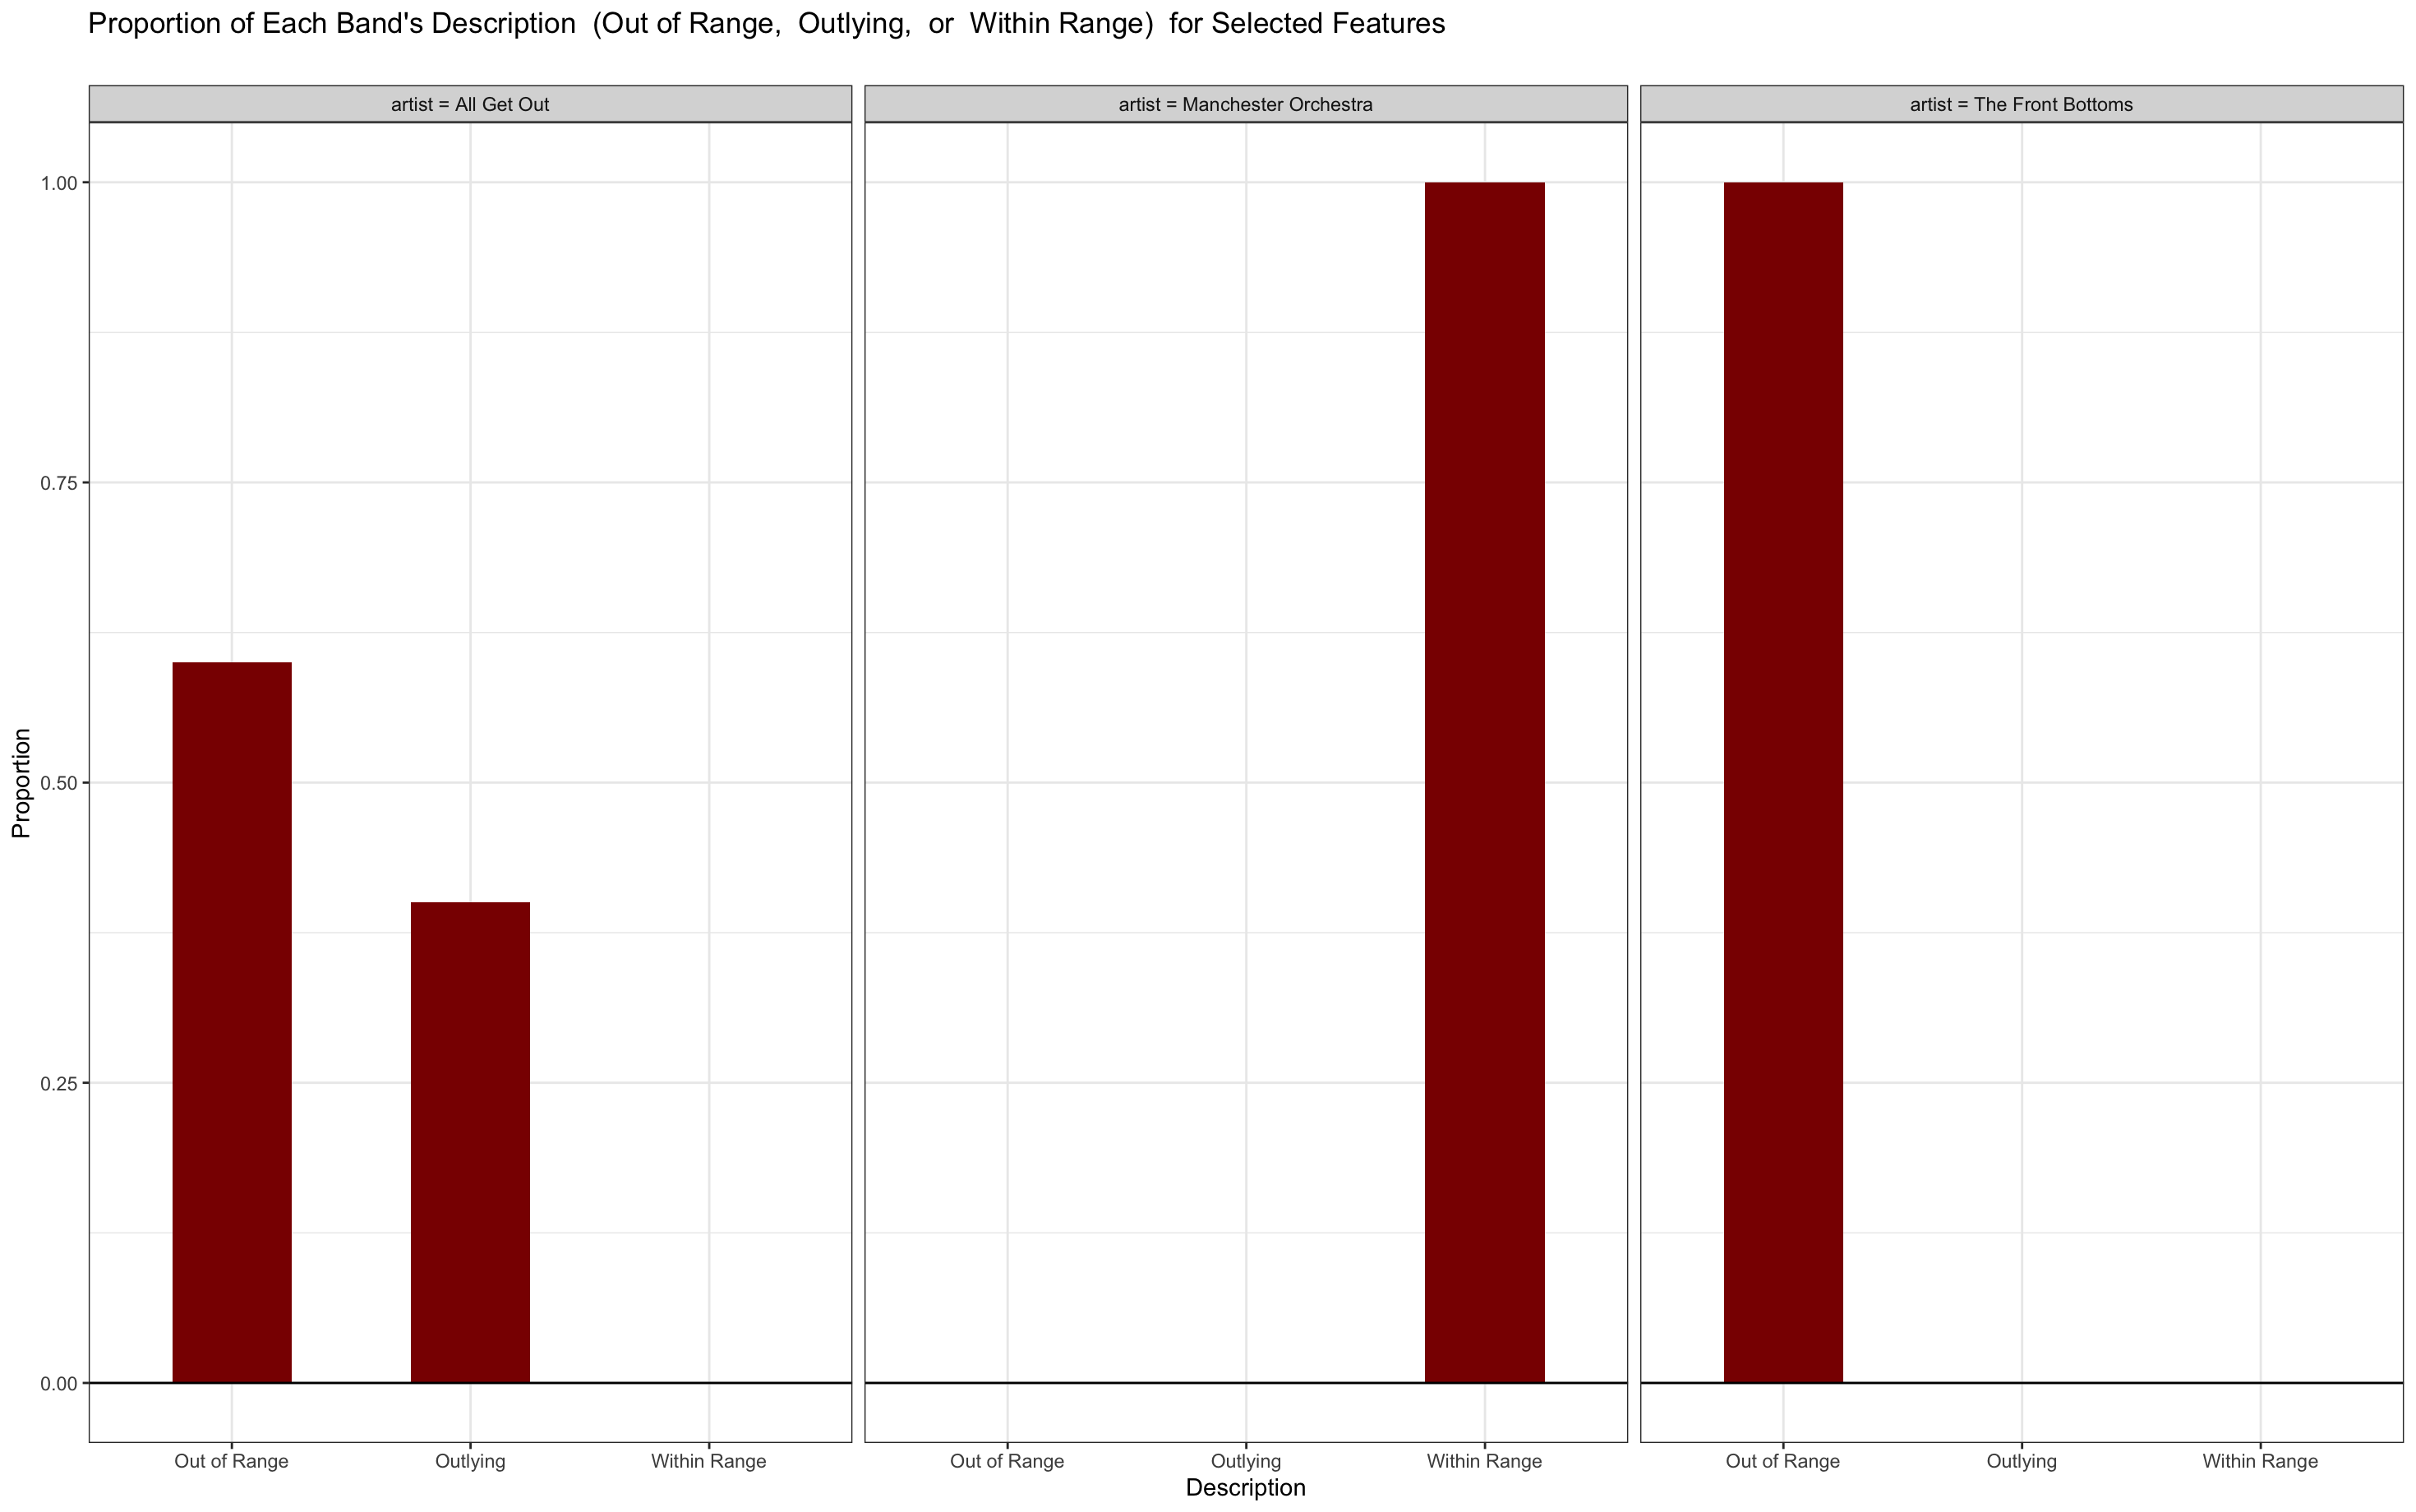
\includegraphics[width=1.05\textwidth, trim=0 0 0 50, clip]{bar.png}
    \caption{Proportion of Each Band's Description  (Out of Range,  Outlying,  or  Within Range)  for Selected Features}
    \vspace{0.20cm} 
    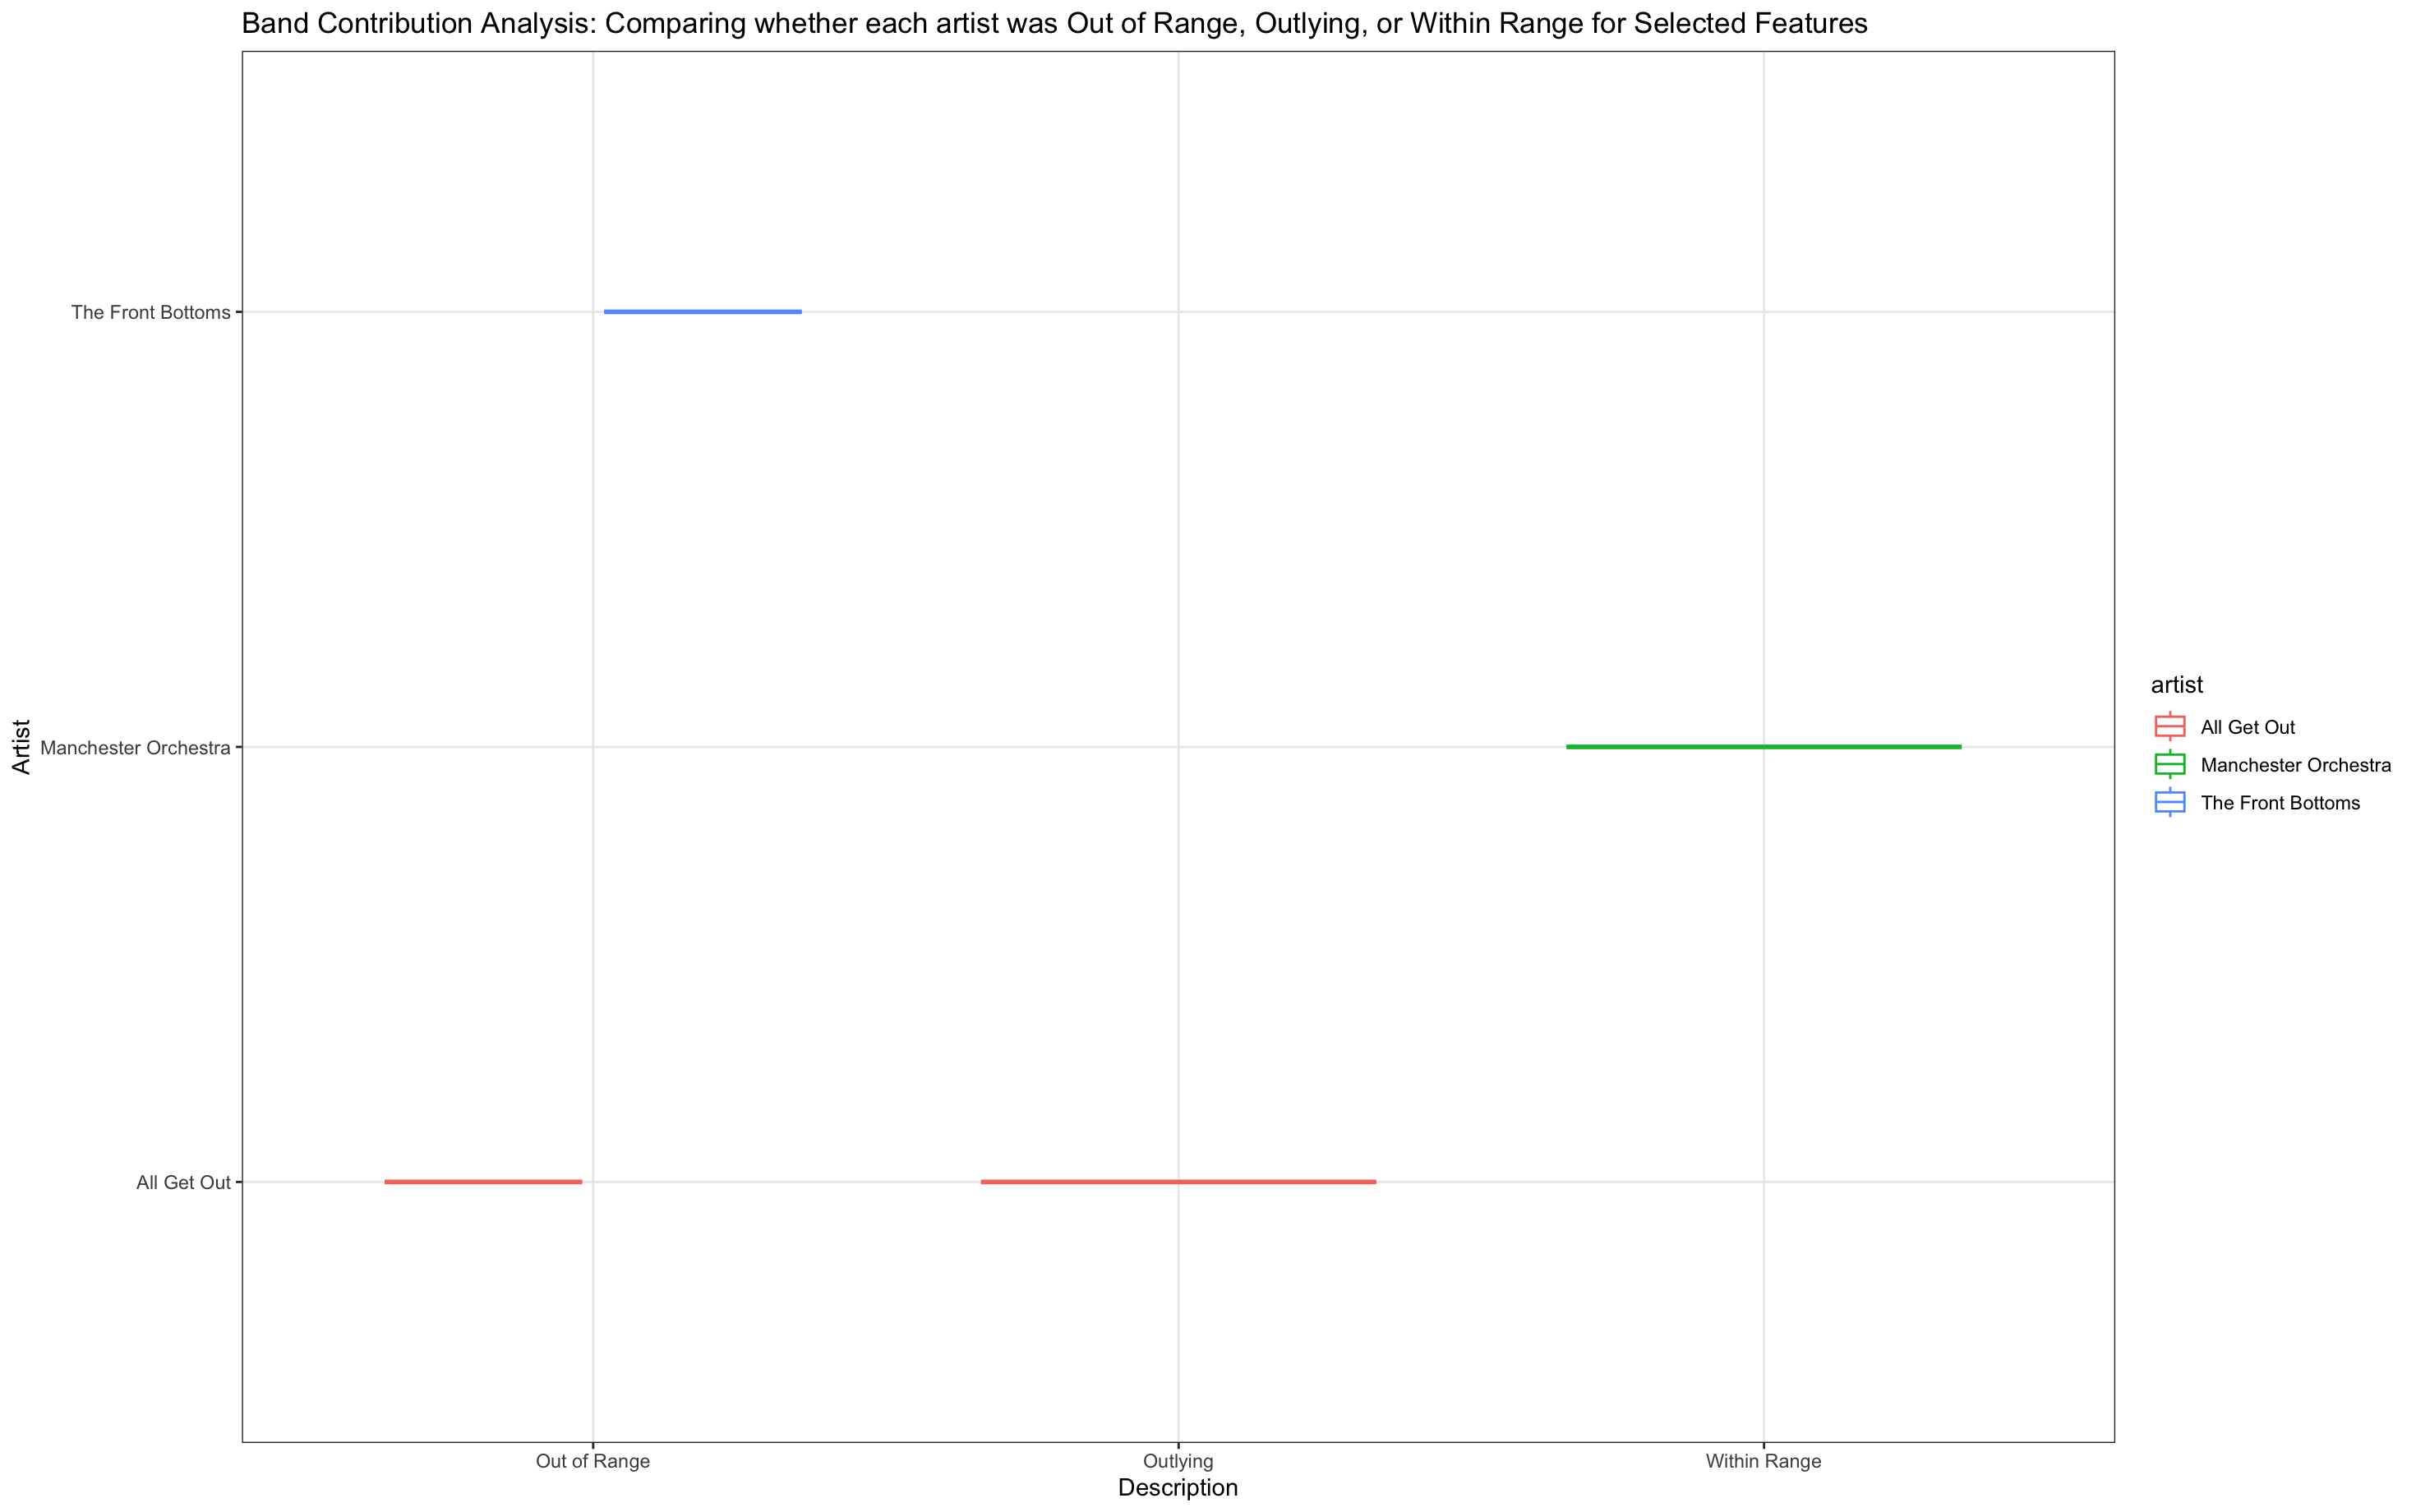
\includegraphics[width=1.05\textwidth, trim=0 0 0 50, clip]{Plot.png}
    \caption{Each Description's Distribution Between All Artists}
\end{figure}


\end{document}
